GeneNet VR has room for improvements and new ideas. During the development, I used a git repository hosted on GitHub. I used the issues list that GitHub offers in order to have an overview of the problems that the application had. There are still a few issues opened and that I didn't have time to work with; some are bugs and others are ideas for future development. The project is now open source and anyone can contribute to it. The repository can be found in this URL on my GitHub account \footnote{https://github.com/kolibrid/GeneNet-VR}. The issue list can be found in this URL  \footnote{https://github.com/kolibrid/GeneNet-VR/issues}.

As we can see in the list, there are some issues that are tagged as "bug"; These bugs are not very big and don't prevent GeneNet VR from being functional. However, they have some impact upon the usability of the application.

A problem that we found out is that when the application is run on the Oculus Quest hardware, the pointer for the 2D menu dones't work. With this problem, the user cannot use the filters or the morph slider. Also when we morph the datasets, the new position of the networks are not taken into account if they have been translated previously. Other small bugs are that there seems to be an offset in the teleportation arrow, so the user doesn't teleport exacly to the direction of the arrow; also sometimes the pointer selects nodes that are behind the users, and it should be only the ones that are in front of the user.

We believe that GeneNet VR has also potential for new development. We have written som ideas and tagged them with the word "enhancement" on GitHub. Something that could be interesting is to make the application mulituser. We got this idea from CellexalVR\cite{cellexalvr}, where two people can be in the same session and only one of them can interact with the data, the other is only a watcher. We could implement something similar in GeneNet VR, where one of the users is just a watcher but can for instance teleport to other parts of the network to visualize it.

Another improvement that we think that would enhance the performance of the application, is to create the lines that correspond to the edges during the initialization of the application and show them when they are needed. Right now, these lines are created in the scene every time a new node is selected. We use a function from Unity called Instantiate for this, which can downgrade the performance of the application, according to some forums from Unity.

Other improvements for BigNet VR would be focused on teh aesthetics of the application. It's something that we haven't focused much in our prototype. An issue that we can see is that the nodes that we filter and that are morphed are turned into a black colour. It would be better to make the nodes transparent or to remove them from the network (when we filter them). If the nodes are still there but in black colour, they could hide other nodes that are behind them and the user might not see those nodes.

Other ideas that we had to improve GeneNet VR are for example hightlight the nodes that are selected and their related nodes, the possibility to adjust the space between the nodes in the clusters and improve the 2D elements like the menu.

Finally, we would also like to run other experiments to further evaluate the performance of the application and study better the scalability. We would like to use larger datasets in order to determine where is the size limit for which we can visualize these datasets in GeneNet VR for both PC and the Oculus Quest headset.

\section{New requirements based on the interviews}
\begin{figure}[h!]
    \setlength{\tempheight}{15ex}
    \centering
    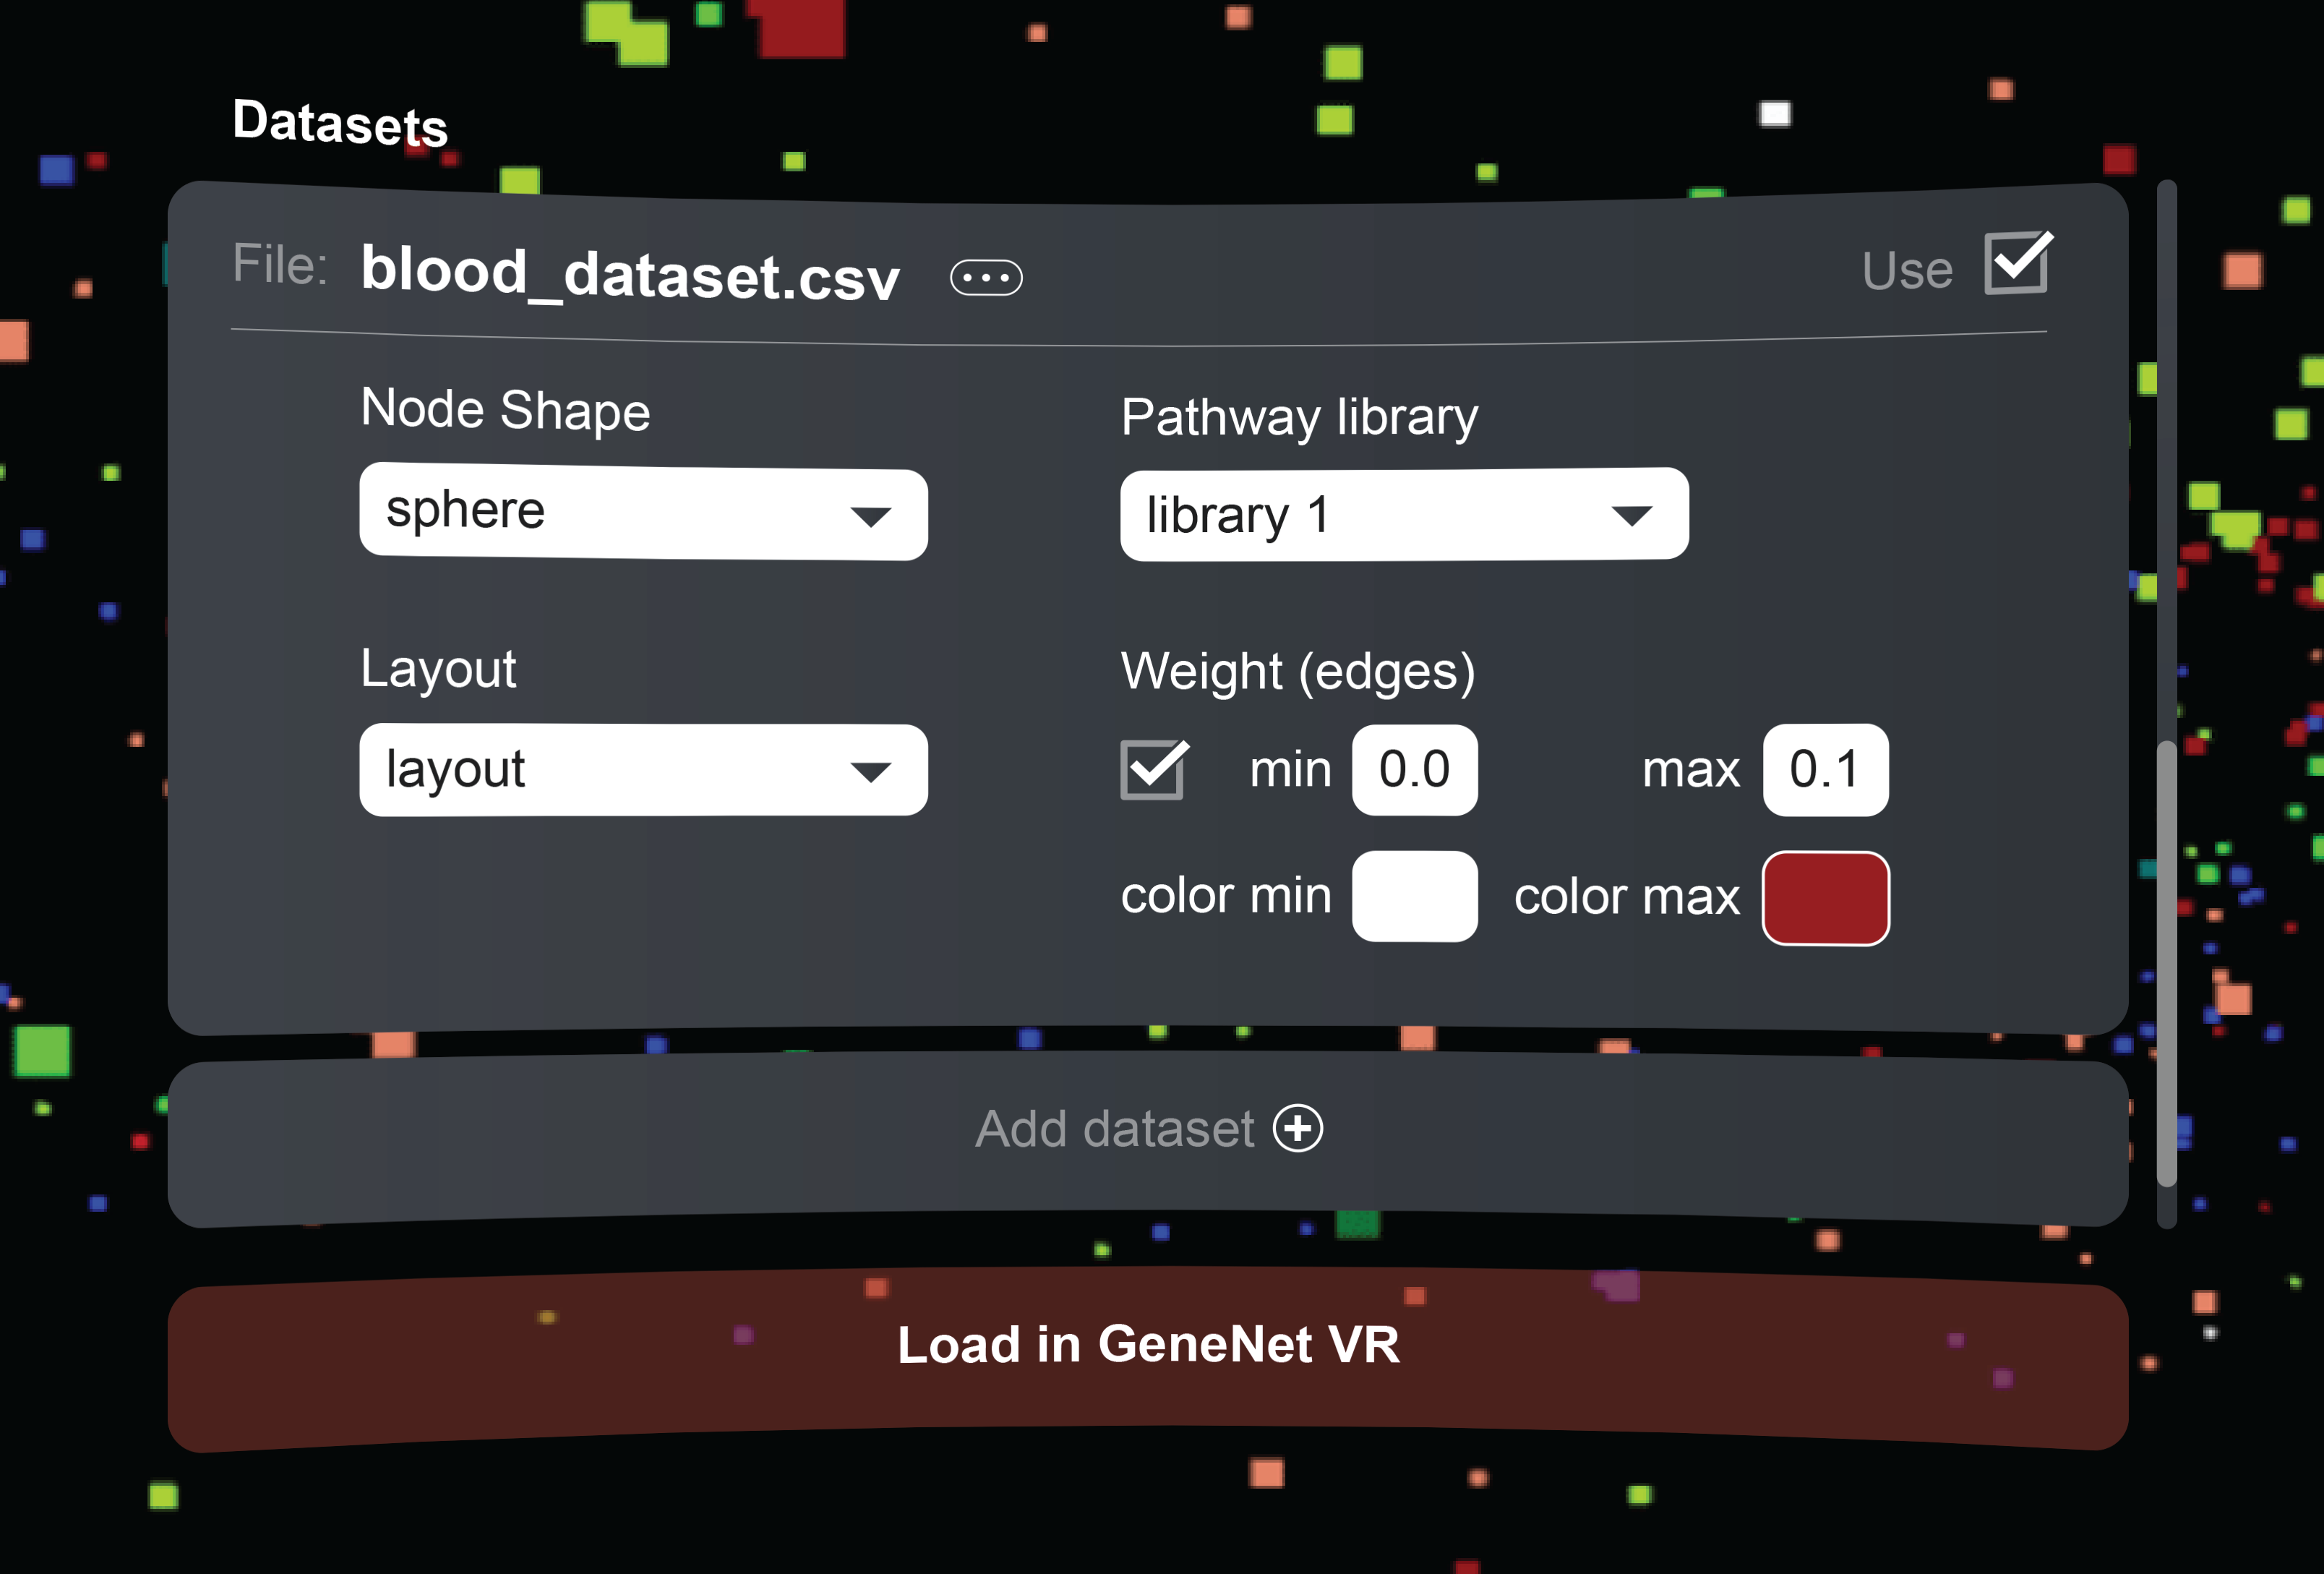
\includegraphics[width=\textwidth]{ui_future}
    \caption{Design of a user interface for GeneNet VR with help of a graphic designer.}
    \label{fig:issues}
\end{figure}

We obtained very interesting feedback from the interviews. We have created a list of issues based on this feedback and tagged them with the workd "interviews" on GitHub.

Some respondants from the interviews who work on biology research projects claimed that it would be helpful to also see the names of the nodes that are interconnected to the selected node. When we select a node, we only get information for the node name that we have selected, but not for the interconnected nodes. A solution to this is be to show a text label on the interconnected nodes or a small window with the interconnected node names. This task is tricky because we can end up having a lot of information. We can also try to highlight the nodes that we are visualizing and show the name labels when we get close to the nodes.

There is also information in the edges that we are not showing, like the weights. This information is common in networks like co-expression gene, social and drug networks. We can show the weight values by using a colour range in the lines or by changing the thickness of these. The distance between one and another node can also give important information about this.

Other improvements that we would ike to do based on the interviews is: to be able to rotate the network with the controllers, filter the nodes by clusters, use a node search functionality, make the snap rotation smoother, be able to pin a node to compare it with other nodes and make it easier to select nodes by showing a collision circle around the nodes.

We also discussed the idea of building a notebook interface where the bioinformaticians can edit the datasets before uploading them to GeneNet VR. A notebook interface is a virtual notebook environment used for literate programming. It's a word processing tool where we also have a shell and kernel of a programming language. Notebooks are very useful to analyze data. The idea would be that the users can edit the dataset by changing the layout, using a different pathway library, changing the co-expression limit, adding other nodes, etc. then GeneNet CR is used to visualize the dataset by using the interaction functionalities.

Finally, we have created an improved user interface with some UI elements for GeneNet VR with help of a graphic designer, as we can see in Figure \ref{fig:issues}. These UI elements could be used in other parts of GeneNet VR like the filtering menu, a node search menu or to edit properties of the current network, to cite some examples.
